\documentclass{article}
\usepackage[utf8]{inputenc}
\usepackage{graphicx}
\graphicspath{ {./Images/} }
\usepackage{url}
% By default the URLs are put in typewriter type in the body and the
% bibliography of the document when using the \url command.  If you are
% using many long URLs you may want to uncommennt the next line so they
% are typeset a little smaller.
\renewcommand{\UrlFont}{\small\tt}


\title{A Comparative Study Of Brain Computer Interface Algorithms: SVM Classifiers vs Neural Networks}
\author{Krishna Vijay Samayamantri}
\date{November 2018}

\begin{document}

\maketitle

\newpage
%%%%%%%%%%%%%%%%%%%%%%%%%%%%%%%%%%%%%%%%%%%%%%%%%%%%%%
%%%%%%           List of Figures                %%%%%%
%%%%%%%%%%%%%%%%%%%%%%%%%%%%%%%%%%%%%%%%%%%%%%%%%%%%%%
\listoffigures 
%%%%%%%%%%%%%%%%%%%%%%%%%%%%%%%%%%%%%%%%%%%%%%%%%%%%%%
%%%%%%           List of Tables                 %%%%%%
%%%%%%%%%%%%%%%%%%%%%%%%%%%%%%%%%%%%%%%%%%%%%%%%%%%%%%
\listoftables

\newpage
\section{Data Collection}
% Intro to Data Collection
Electroencephalogram (EEG) is the most common method for recording brain signals in humans. This is due to EEG being safe, non-intrusive, easy to use and inexpensive. Also, EEG has a high temporal resolution (of the order of milliseconds)\cite{lotte:hal-01167515} \cite{niedermeyer2005electroencephalography}.
Most BCI systems use Event Related Potentials (ERP's) to control an external system. Event Related Potentials (ERP's) are stereotyped deflections of the EEG, related to a sensory, cognitive or motor event. The “Event” of an ERP must come at a precise measurable time, called the time trigger of the event. Typically, if a person is receiving a sensory stimulus, the time trigger is the instant at which the stimulus is presented, or, in case of a button press, it is the instant at which the muscular activity exceeds a certain threshold.
% Dunno if this sentence below can be removed
The deflections measured by the ERP's are represented as waveforms, and sometimes called waves.\cite{lotte:hal-01167515}

% Physical Setup
\subsection{Experimental Setup}
For our data collection, we have used the Emotiv EPOC+ BCI device coupled with EmotivPRO,  the corresponding software. Through our setup, we were able to collect EEG data with markers indicating the occurrence of each "event" in order to obtain ERP's. 

% Emotiv EPOC+
\subsubsection{Emotiv EPOC+}
Emotiv EPOC+ (Shown in \ref{fig:EPOC}) is a commercially available EEG-based BCI device manufactured by Emotiv Inc. Emotiv EPOC is wireless, portable, inexpensive (compared to medical grade EEG devices), and is quick and easy to setup and remove.\cite{EPOCUserManual:2018} 

There are a total of 14 EEG sensors and two reference electrodes on the Emotiv EPOC+. They are labelled as follows: AF3, F7, F3, FC5, T7, P7, O1, O2, P8, T8, FC6, F4, F8, AF4 plus 2 reference electrodes: CMS and DRL corresponding to P3 and P4 as shown in \ref{fig:Electrode Mapping}.

% Emotiv EPOC+ Image
\begin{figure}[tbp]
    \centering
    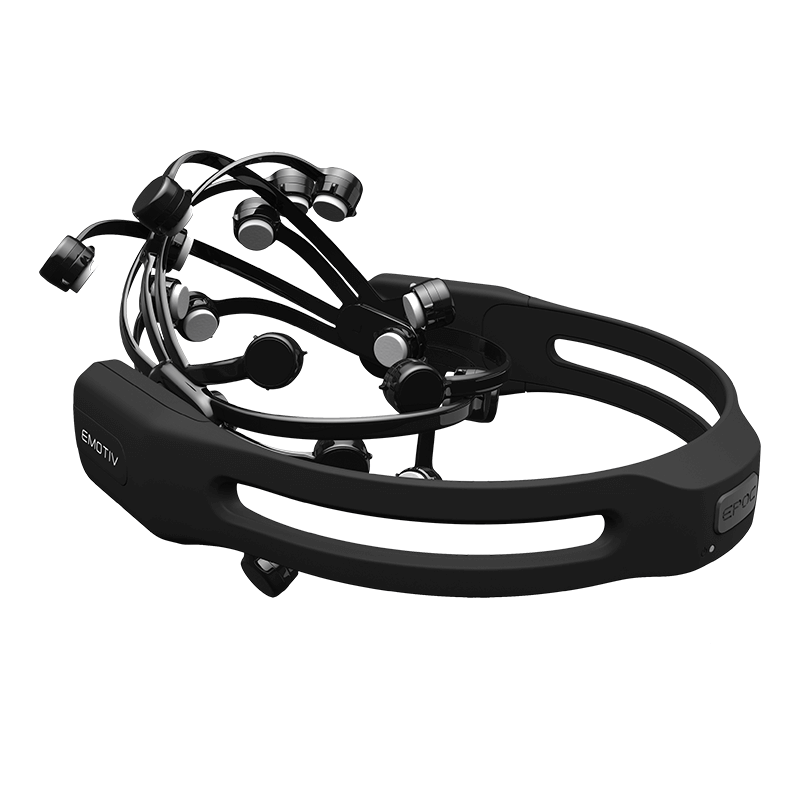
\includegraphics[scale = 0.25]{Images/Epoc-product-image.png}
    \caption{Emotiv EPOC+}
    \label{fig:EPOC}
\end{figure}

% Emotiv Electrode Mapping over International 10-20 EEG System
\begin{figure}[tbp]
    \centering
    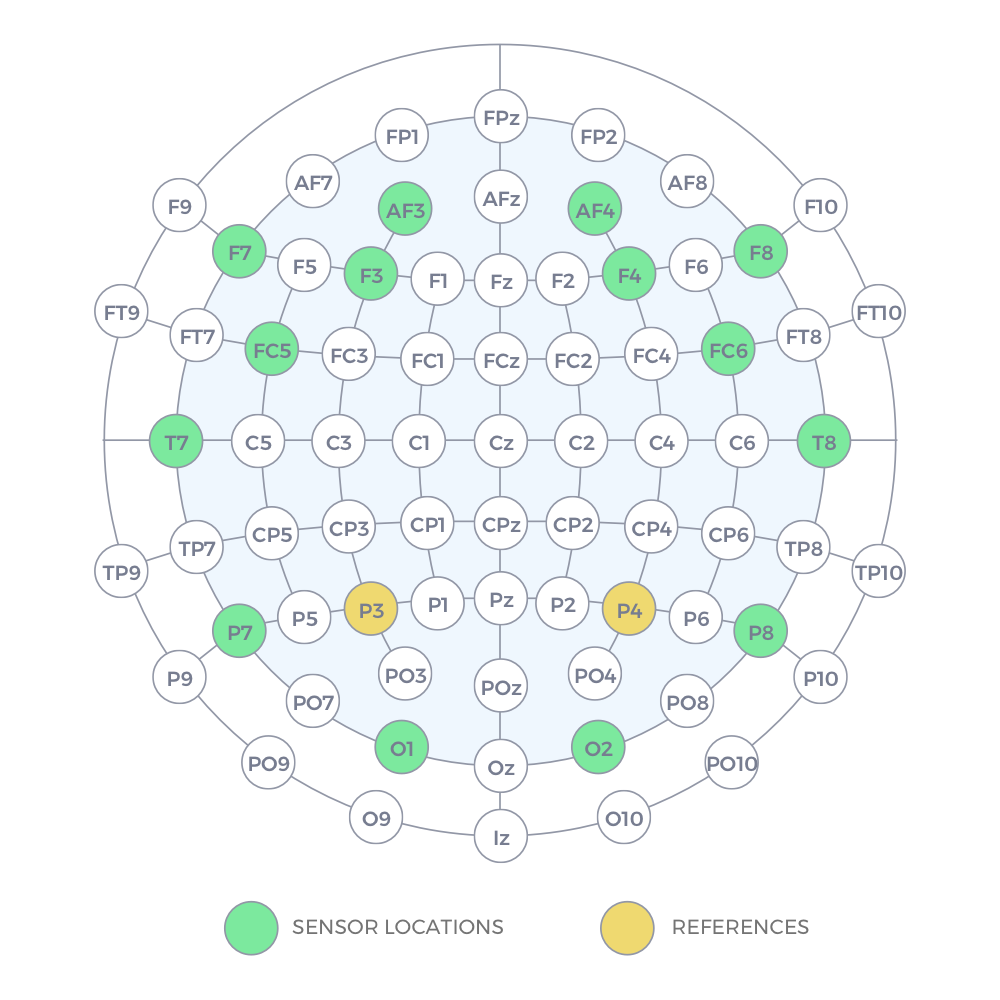
\includegraphics[scale = 0.25]{Images/epoc-20-10.jpg}
    \caption{EPOC+ Electrode Mapping over International 10-20 EEG System}
    \label{fig:Electrode Mapping}
\end{figure}

% Emotiv EPOC Specifications
Table \ref{tab:Emotiv Specs} lists the technical specifications of the EPOC+ used.
\begin{table}[htbp]
    \centering
    \begin{tabular}{|p{7cm}|p{7cm}|}
        \hline
         No. of Channels & 14 (plus CMS/DRL references, P3/P4 locations) \\ [1ex]
        \hline
         Channel names (International 10-20 locations) & AF3, F7, F3, FC5, T7, P7, O1, O2, P8, T8, FC6, F4, F8, AF4 \\[1ex]
        \hline
         Sampling method & Sequential sampling. Single ADC \\ [1ex]
        \hline
         Sampling rate & 128 SPS / 256 SPS (2048 Hz internal) \\ [1ex]
        \hline
         EEG Resolution & 14 bits 1 LSB = 0.51$\mu$V (16 bit ADC, 2 bits instrumental noise floor discarded) Settings can be changed to 16-bit  \\ [1ex]
        \hline
         Bandwidth & 0.2 - 45Hz, digital notch filters at 50Hz and 60Hz \\ [1ex]
        \hline
         Filtering & Built in digital 5th order Sinc filter \\ [1ex]
        \hline
         Dynamic range (input referred) & 8400 $mu$V(pp) \\ [1ex]
        \hline
         Coupling mode & AC coupled \\ [1ex]
        \hline
         Connectivity & Proprietary 2.4GHz wireless, BLE and USB \\ [1ex]
        \hline
         Battery Capacity & LiPo battery 680mAh \\ [1ex]
        \hline
         Battery life (typical) & 12 hours \\ [1ex]
        \hline
         Impedance Measurement & Real-time contact quality using patented system \\ [1ex]
        \hline
         IMU Part & ICM-20948 \\ [1ex]
        \hline
         Accelerometer & 3-axis +/-8g \\ [1ex]
        \hline
         Gyroscope & 3-axis +/- 2000 dps \\ [1ex]
        \hline
         Magnetometer & 3-axis +/- 12 gauss \\ [1ex]
        \hline
         MEMS Sampling & 32 / 64 / 128 Hz (User Defined) \\ [1ex]
        \hline
         MEMS Resolution & 16-bit \\ [1ex]
        \hline
         Sensor Material & Ag/AgCl + Felt + Saline \\ [1ex]
         \hline
    \end{tabular}
    \caption{Emotiv EPOC+ Technical Specifications}
    \label{tab:Emotiv Specs}
\end{table}
 
% Emotiv PRO
\subsubsection{EmotivPRO}
The EmotivPRO software is used to collect raw EEG data. It offers a graphical representation of EEG signals which can be recorded and saved. Also, EmotivPRO provides user the facility to mark events based on a keystroke marker or markers sent via com port. Figure \ref{fig:EmotivPRO with Markers} shows screen-shot of EmotivPRO with markers.

% Emotiv PRO with Markers
\begin{figure}[tbp]
    \centering
    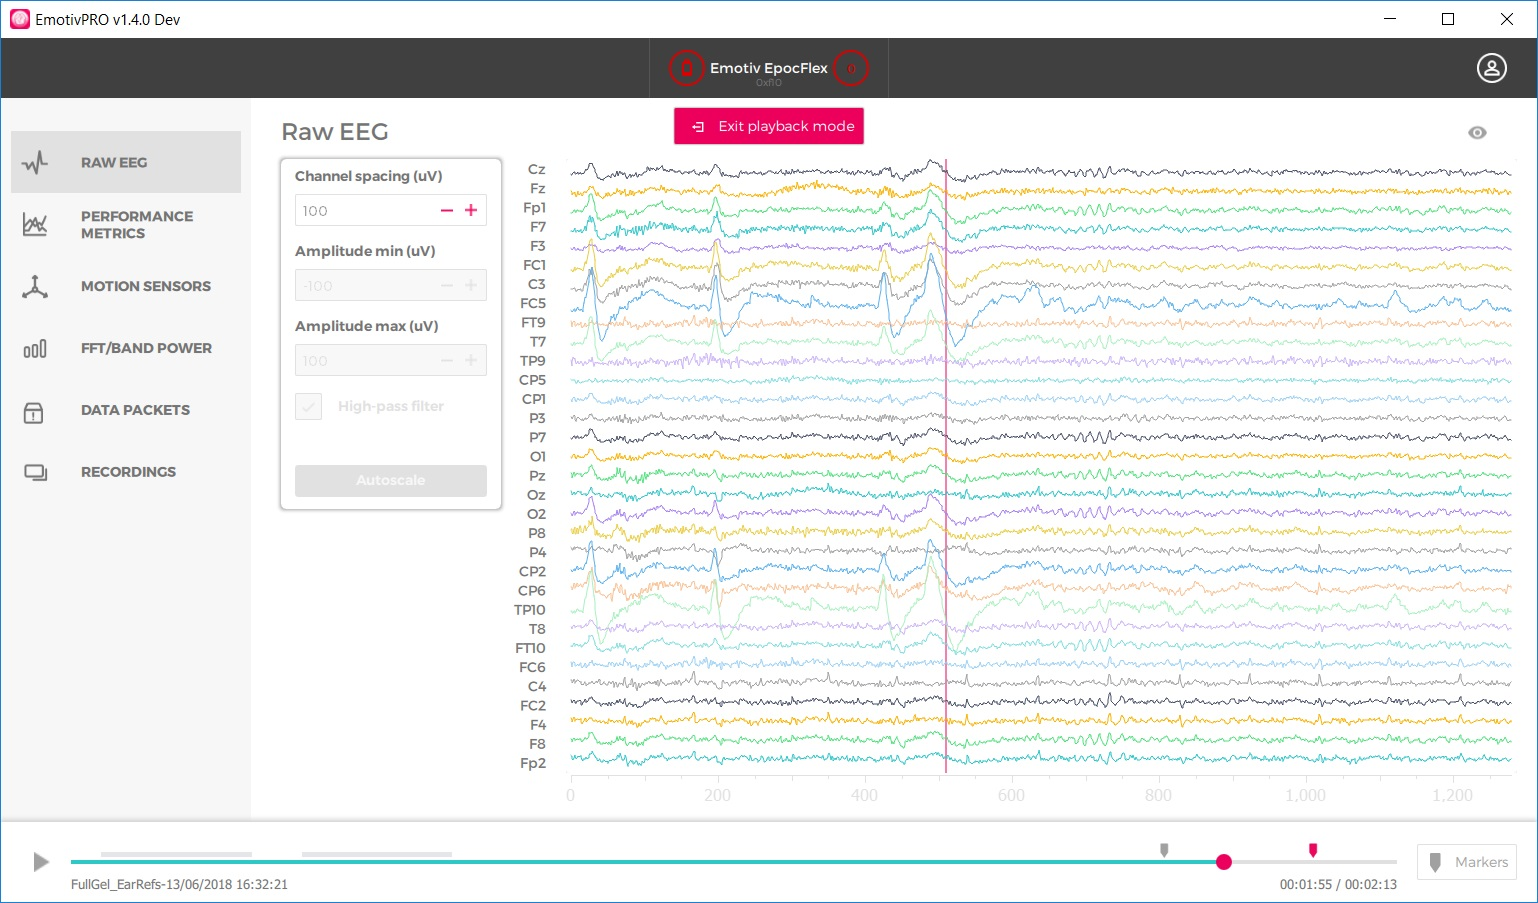
\includegraphics[scale=0.3]{Images/EmotivPRO-Markers.jpg}
    \caption{EmotivPRO with Markers}
    \label{fig:EmotivPRO with Markers}
\end{figure}

% Experiment Details
\subsubsection{Experiment Details}
Initially, we tried to record EEG using manual keystroke markers. In initial data collection sessions, we had a user move the mouse cursor across the display along a horizontal blue line upon hearing an audio cue \textbf{"GO"} from the experimenter. It consisted of three parts: \textbf{Ready, Action and Rest.} At the start of each session, the mouse cursor is reset and the user sits relaxed with their hands resting on the table. In \textbf{Ready}, the subject sits with their hand resting on the mouse, relaxed and readily waiting for the instruction \textbf{"GO."}

% Mouse Cursor Movement Experiment
\begin{figure}[tbp]
    \centering
    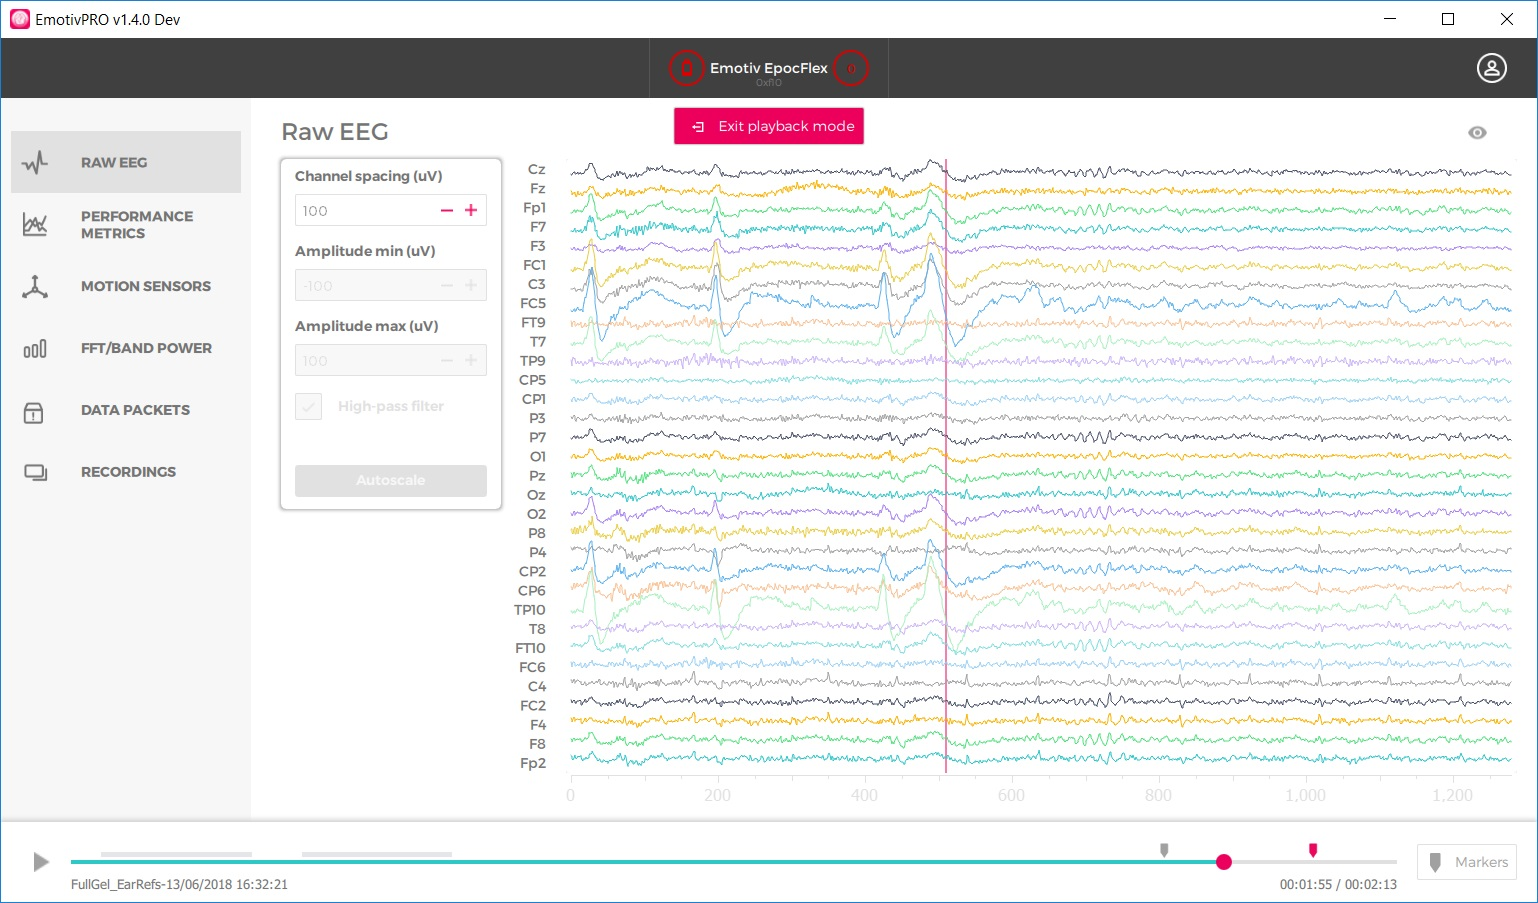
\includegraphics[scale=0.3]{Images/EmotivPRO-Markers.jpg}
    \caption{Mouse Cursor Movement Experiment}
    \label{fig:EmotivPRO with Markers}
\end{figure}

We have created a simple test that records the subject's EEG for motor intent and motor action. Each subject is asked to sit on a chair with their hands resting on a table in front of them. They are asked to look at a computer screen that shows them cues for each event. First, they get the cue 'Relax' which tells them to relax and be still. After 5 seconds, they get the cue 'Ready Left' or 'Ready Right' randomly. The subject is supposed to imagine the motor intent that they are going to perform after 5 seconds, which is touch an object placed on the table with the chosen hand. Finally, they get the cue 'Reach' when they reach out with the chosen hand and actually touch the object (Shown in Figure \ref{fig:Experimental Setup}). A simple LabVIEW program (Shown in Figure \ref{fig:LabVIEW Light Sequence}) is created that displays the cue for each event and sends corresponding markers to EmotivPRO via com port. This program also sends a marker indicating 'end of cycle.' The program repeats the cycle 50 times for each session.

% Experimental Setup
\begin{figure}[tbp]
    \centering
    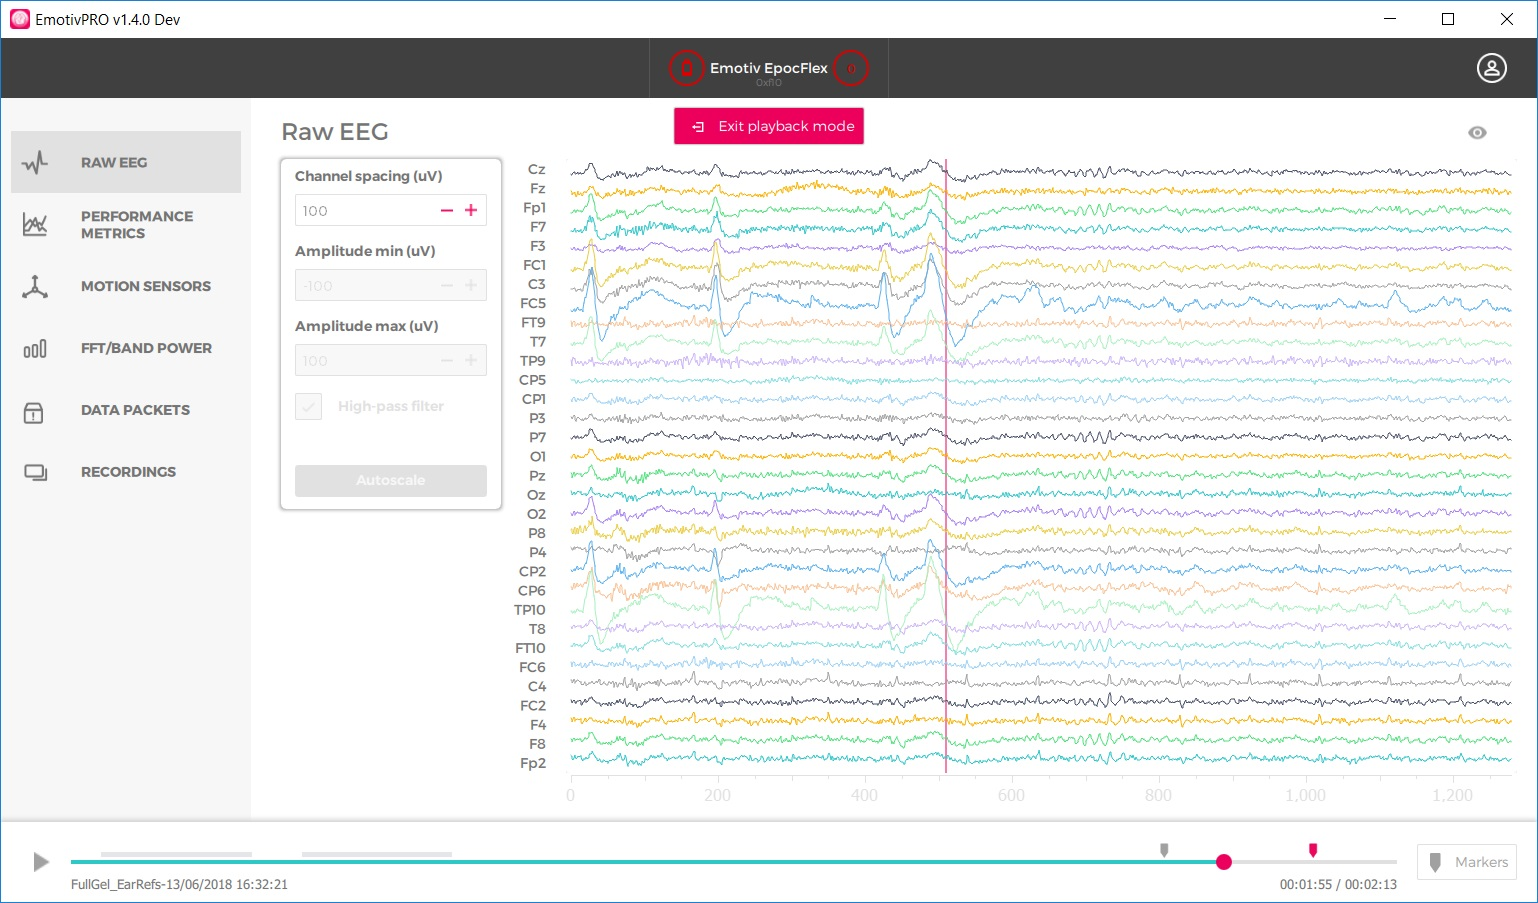
\includegraphics[scale=0.3]{Images/EmotivPRO-Markers.jpg}
    \caption{Experimental Setup}
    \label{fig:Experimental Setup}
\end{figure}

% LabVIEW Light Sequence Program
\begin{figure}[tbp]
    \centering
    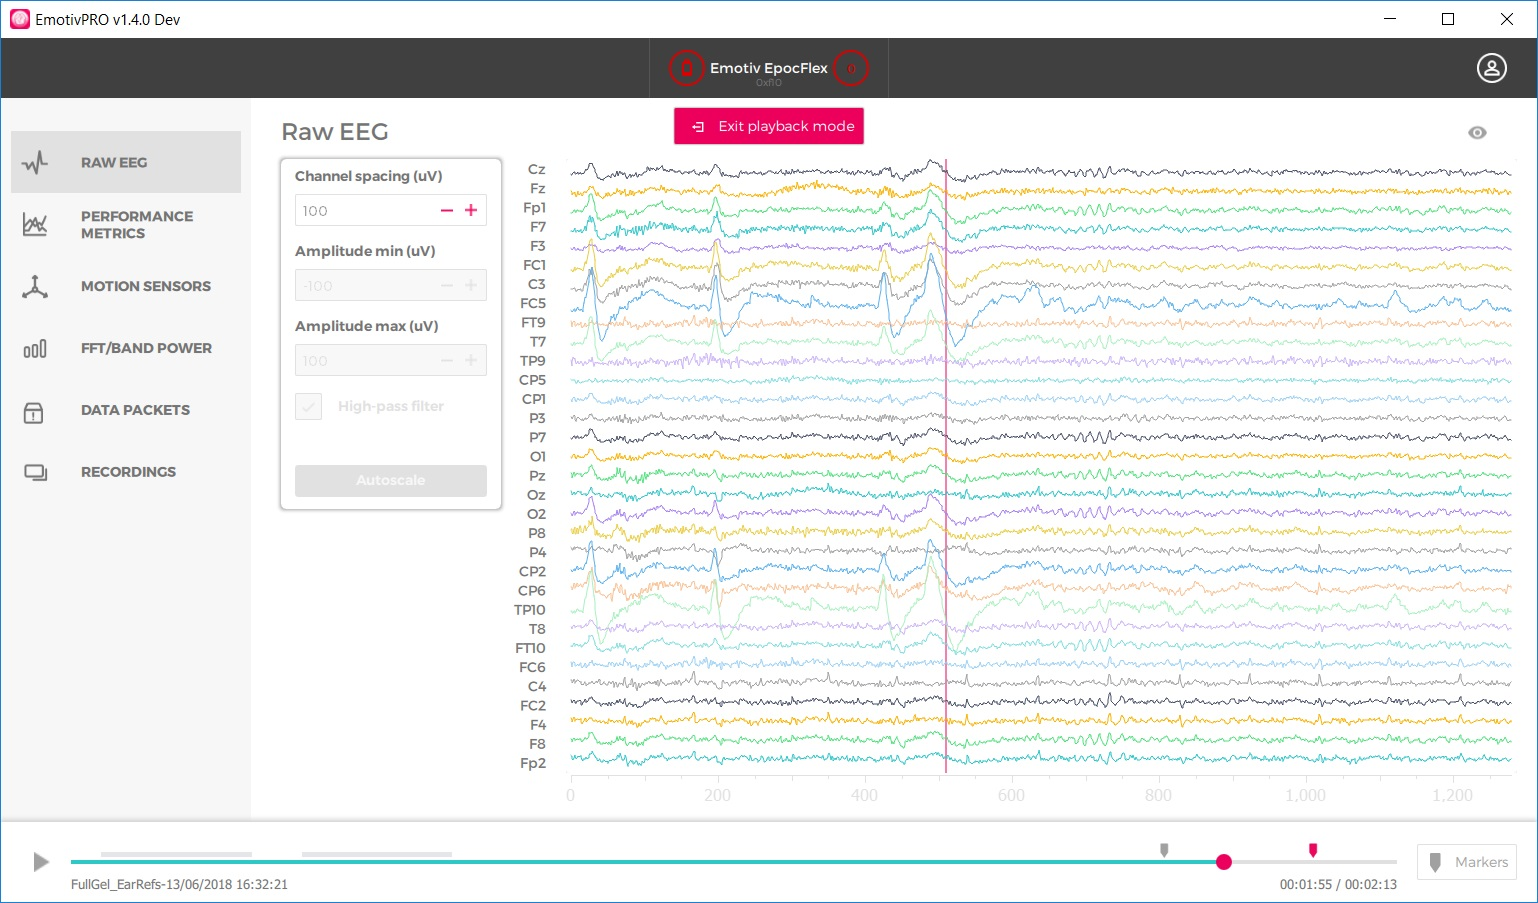
\includegraphics[scale=0.3]{Images/EmotivPRO-Markers.jpg}
    \caption{LabVIEW Light Sequence}
    \label{fig:LabVIEW Light Sequence}
\end{figure}


% Physionet Dataset
\subsection{Physionet Dataset}

%%%%%%%%%%%%%%%%%%%%%%%%%%%%%%%%%%%%%%%%%%%%%%%%%%%%%%
%%%%%%              References                  %%%%%%
%%%%%%%%%%%%%%%%%%%%%%%%%%%%%%%%%%%%%%%%%%%%%%%%%%%%%%
\newpage
\bibliographystyle{ieeetr} % IEEE Reference Style
\bibliography{References} % BibTEX file name where references are listed


% In final draft I shall put list of figures at the top of the document as required

\end{document}
